%%%%%%%% ICML 2021 EXAMPLE LATEX SUBMISSION FILE %%%%%%%%%%%%%%%%%
\PassOptionsToPackage{table,xcdraw}{xcolor}
\documentclass{article}

% Recommended, but optional, packages for figures and better typesetting:
\usepackage{microtype}
\usepackage{tcolorbox} % For creating colored boxes
\usepackage{amsmath} % For mathematical expressions
\usepackage{graphicx}
% \usepackage{subfigure}
\usepackage{booktabs} % for professional tables
% \usepackage[table,xcdraw]{xcolor}

% hyperref makes hyperlinks in the resulting PDF.
% If your build breaks (sometimes temporarily if a hyperlink spans a page)
% please comment out the following usepackage line and replace
% \usepackage{icml2021} with \usepackage[nohyperref]{icml2021} above.
\usepackage{hyperref}

% Attempt to make hyperref and algorithmic work together better:
\newcommand{\theHalgorithm}{\arabic{algorithm}}

% Use the following line for the initial blind version submitted for review:
%\usepackage{icml2021}
\usepackage{subcaption}
\newcommand{\todo}[1]{\textcolor{red}{}}
\newcommand{\todoshiv}[1]{\textcolor{red}{@Shiv: #1}}
\newcommand{\todogx}[1]{\textcolor{red}{@GX: #1}}
\newcommand{\todoisha}[1]{\textcolor{purple}{@Isha: #1}}
\newcommand{\todokai}[1]{\textcolor{blue}{@Kai: #1}}

% \usepackage{algorithm}
\usepackage{algpseudocode}
\usepackage{amsfonts}
\newcommand{\Figref}[1]{Figure~\ref{#1}}
\newcommand{\figref}[1]{Figure~\ref{#1}}
\newcommand{\Tabref}[1]{Table~\ref{#1}}
\newcommand{\tabref}[1]{Table~\ref{#1}}
\newcommand{\Secref}[1]{Section~\ref{#1}}
\newcommand{\secref}[1]{Section~\ref{#1}}
\newcommand{\Algref}[1]{Algorithm~\ref{#1}}
\renewcommand{\algref}[1]{Algorithm~\ref{#1}}
\newcommand{\appref}[1]{Appendix~\ref{#1}}
\newcommand{\Appref}[1]{Appendix~\ref{#1}}

\newenvironment{tightlist}{
\begin{list}{$\bullet$}{
%    \setlength{\topsep}{0in}
    \setlength{\topsep}{.1em}
    \setlength{\partopsep}{0in}
    \setlength{\parskip}{0in}
    \setlength{\itemsep}{0in}
    \setlength{\parsep}{0in}
    % \setlength{\leftmargin}{1.5em}
    \setlength{\leftmargin}{1em}
    \setlength{\rightmargin}{0in}
    \setlength{\itemindent}{0in}
}}
{\end{list}}

% \newenvironment{tightenum}{
% \begin{enumerate}
% %    \setlength{\topsep}{0in}
%     \setlength{\topsep}{.1em}
%     \setlength{\partopsep}{0in}
%     \setlength{\parskip}{0in}
%     \setlength{\itemsep}{0in}
%     \setlength{\parsep}{0in}
%     % \setlength{\leftmargin}{1.5em}
%     \setlength{\leftmargin}{1em}
%     \setlength{\rightmargin}{0in}
%     \setlength{\itemindent}{0in}
% }
% {\end{enumerate}

\usepackage{tikz}
\usetikzlibrary{calc, shapes, arrows, positioning}
\usetikzlibrary{bayesnet}
% If accepted, instead use the following line for the camera-ready submission:
\usepackage[accepted]{icml2021}



% The \icmltitle you define below is probably too long as a header.
% Therefore, a short form for the running title is supplied here:
\icmltitlerunning{A Probabilistic Inference Approach to Inference-Time Scaling of LLMs using Particle-Based Monte Carlo Methods}

\begin{document}

\twocolumn[
\icmltitle{A Probabilistic Inference Approach to Inference-Time Scaling of LLMs using Particle-Based Monte Carlo Methods}

% It is OKAY to include author information, even for blind
% submissions: the style file will automatically remove it for you
% unless you've provided the [accepted] option to the icml2021
% package.

% List of affiliations: The first argument should be a (short)
% identifier you will use later to specify author affiliations
% Academic affiliations should list Department, University, City, Region, Country
% Industry affiliations should list Company, City, Region, Country

% You can specify symbols, otherwise they are numbered in order.
% Ideally, you should not use this facility. Affiliations will be numbered
% in order of appearance and this is the preferred way.
\icmlsetsymbol{equal}{*}

\begin{icmlauthorlist}

\icmlauthor{Isha Puri}{mit}
\icmlauthor{Shivchander Sudalairaj}{rh-ibm}
\icmlauthor{Guangxuan Xu}{rh-ibm}
\icmlauthor{Kai Xu}{rh-ibm}
\icmlauthor{Akash Srivastava}{rh-ibm}

\icmlauthor{$^1$ MIT CSAIL}{}
\icmlauthor{$^2$ Red Hat AI Innovation}{}


\end{icmlauthorlist}

\icmlaffiliation{mit}{MIT CSAIL}
\icmlaffiliation{rh-ibm}{Red Hat AI Innovation}


\icmlcorrespondingauthor{Isha Puri}{ishapuri@mit.edu}
\icmlcorrespondingauthor{Shivchander Sudalairaj}{ssudalai@redhat.com}


% You may provide any keywords that you
% find helpful for describing your paper; these are used to populate
% the "keywords" metadata in the PDF but will not be shown in the document
\icmlkeywords{Machine Learning, ICML}

\vskip 0.3in
]

% this must go after the closing bracket ] following \twocolumn[ ...

% This command actually creates the footnote in the first column
% listing the affiliations and the copyright notice.
% The command takes one argument, which is text to display at the start of the footnote.
% The \icmlEqualContribution command is standard text for equal contribution.
% Remove it (just {}) if you do not need this facility.

%\printAffiliationsAndNotice{}  % leave blank if no need to mention equal contribution

\printAffiliationsAndNotice{\textsuperscript}
\begin{abstract}
Large language models (LLMs) have achieved significant performance gains via scaling up model sizes and/or data. 
However, recent evidence suggests diminishing returns from such approaches, motivating scaling the computation spent at inference time. 
Existing inference-time scaling methods, usually with reward models, cast the task as a search problem, which tends to be vulnerable to reward hacking as a consequence of approximation errors in reward models.
In this paper, we instead cast inference-time scaling as a probabilistic inference task and leverage sampling-based techniques to explore the typical set of the state distribution of a state-space model with an approximate likelihood, rather than optimize for its mode directly.
We propose a novel inference-time scaling approach by adapting particle-based Monte Carlo methods to this task.
Our empirical evaluation demonstrates that our methods have a 4--16x better scaling rate over our deterministic search counterparts on various challenging mathematical reasoning tasks. 
Using our approach, we show that Qwen2.5-Math-1.5B-Instruct can surpass GPT-4o accuracy in only 4 rollouts, while Qwen2.5-Math-7B-Instruct scales to o1 level accuracy in only 32 rollouts.
Our work not only presents an effective method to inference-time scaling, but also connects the rich literature in probabilistic inference with inference-time scaling of LLMs to develop more robust algorithms in future work. Code, videos, and further information available at \href{https://probabilistic-inference-scaling.github.io/}{probabilistic-inference-scaling.github.io/}
. 

%Further, we study various modifications to the computation budget allocation through Particle Gibbs, a Markov chain Monte Carlo method where particle filtering is the transition kernel, as well as Particle Tempering approaches.
\vspace{-1.5em}
\end{abstract}




\section{Introduction}
% OVERALL STORY: imperfections in reward models mean that sampling is beneficial to finding the optimal answer in the search space 

% - extra knobs we can control to further your exploration: 
%     - temperature
%     - parallel particle filtering
%     - particle gibbs (?? if we get this to work )


% typical 1st paragraph about extraordinary development of LLMs, and how inference scaling extends the capabilities of smaller models. More recent inference scaling methods mimic a "thinking / pondering various solutions" process by navigating a wide search space, yadda yadda yadda
% Large language models have been demonstrating increasingly better performance through data scaling and model scaling, in which the key push of frontier models is via collecting more data and increasing the number of learnable parameters \citep{}.
% While such scaling seems to be plateaued in more recently development, the trend of inference-time scaling becomes the new focus to keep improving model performance \citep{}.
% Proprietary models such as OpenAI o1 and o3 have demonstrated the benefits of spending more computation as inference time especially on tasks like math and reasoning.
% Moreover, such techniques not only pushes the model frontiers, but also makes it possible to achieve the same level of performance a large model via inference-time scaling a small model, which is more accessible to various low-resource devices.

\begin{figure}[tt]
    \centering
    \vspace{-1.5em}
    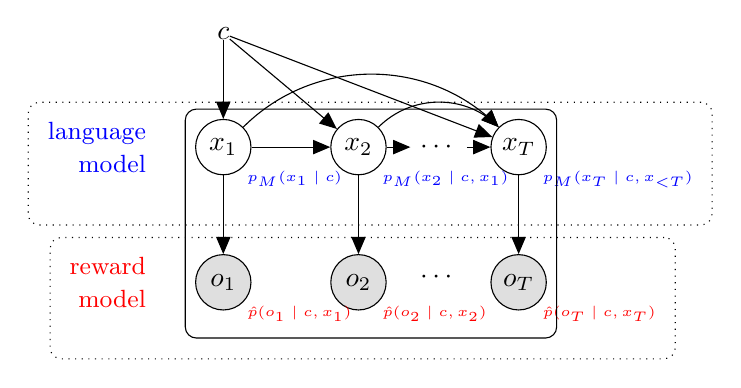
\begin{tikzpicture}
        % Nodes
        \node[latent] (x1) {$x_1$}; 
        \node[latent, right=of x1] (x2) {$x_2$}; 
        \node[right=0.3cm of x2] (dots) {$\cdots$}; 
        \node[latent, right=0.3cm of dots] (xT) {$x_T$}; 

        \node[const, above=of x1] (c) {$c$};

        \node[obs, below=of x1] (o1) {$o_1$}; 
        \node[obs, below=of x2] (o2) {$o_2$}; 
        \node[below=1.25cm of dots] (odots) {$\cdots$}; 
        \node[obs, below=of xT] (oT) {$o_T$}; 

        \node[below right=-0.1cm of x1] (x1p) {\tiny \color{blue} $p_M(x_1 \mid c)$};
        \node[below right=-0.1cm of x2] (x2p) {\tiny \color{blue} $p_M(x_2 \mid c, x_1)$};
        \node[below right=-0.1cm of xT] (xTp) {\tiny \color{blue} $p_M(x_T \mid c, x_{<T})$};
        \node[below right=-0.1cm of o1] (o1p) {\tiny \color{red} $\hat{p}(o_1 \mid c, x_1)$};
        \node[below right=-0.1cm of o2] (o2p) {\tiny \color{red} $\hat{p}(o_2 \mid c, x_2)$};
        \node[below right=-0.1cm of oT] (oTp) {\tiny \color{red} $\hat{p}(o_T \mid c, x_T)$};
        \node[align=right, left=0.5cm of x1] (llm) {\small \color{blue} language\\\small \color{blue} model};
        \node[align=right, left=0.5cm of o1]  (rm) {\small \color{red} reward\\\small \color{red} model};

        % Edges
        \edge {x1} {x2};
        \edge {x2} {dots};
        \edge {dots} {xT};

        \edge {c} {x1};
        \edge {c} {x2};
        \edge {c} {xT};

        \edge {x1} {o1};
        \edge {x2} {o2};
        \edge {xT} {oT};

        % Curly arrows
        \draw[->, bend left=45] (x1) to (xT);
        \draw[->, bend left=45] (x2) to (xT);

        % Plates
        \plate {} {(x1)(x2)(xT)(o1)(o2)(oT)(dots)(odots)} {};
        \plate[dotted] {} {(x1)(x2)(dots)(xT)(llm)(x1p)(x2p)(xTp)} {};
        \plate[dotted] {} {(o1)(o2)(odots)(oT)(rm)(o1p)(o2p)(oTp)} {};

    \end{tikzpicture}
    \caption{State-space model for inference-time scaling. $c$ is a prompt, $x_1, \dots, x_T$ are sequence of partial LLM outputs and $o_1, \dots, o_T$ are the ``observed'' acceptance. We cast inference-time scaling as to estimate the latent states conditioned on $o_t = 1$ for $t=1, 2, \dots, T$, i.e.~all being accepted.}\label{fig:plate}
    \vspace{-1.5em}
\end{figure}

Large language models (LLMs) have demonstrated remarkable improvements in performance through scaling up model sizes and/or data. While frontier models have relied heavily on larger datasets and an ever-increasing number of learnable parameters \citep{kaplan2020scalinglawsneurallanguage,snell2024scalingllm}, smaller LLMs have successfully leveraged domain-specific data to match the performance of larger, general-purpose models \citep{sudalairaj2024lablargescalealignmentchatbots, pareja2024unveilingsecretrecipeguide}. 
However, recent reports indicate plateaus in performance gains through such scaling methods. Consequently, inference-time (aka compute-time / test-time) scaling has emerged as a promising alternative to improve model performance \citep{beeching2024scalingtesttimecompute}. Proprietary models like OpenAI's o1 \cite{openai2024openaio1card} and o3 have demonstrated the benefits of allocating more computation resources at inference time, particularly for complex reasoning and math tasks. These inference-time scaling techniques not only enhance model capability but also allow smaller models to achieve performance levels comparable to their larger counterparts, making advanced AI more accessible for low-resource devices.
% \looseness=-1
\begin{figure*}[t]
    \centering
    
    % First Figure: Llama Models
    % \includegraphics[width=0.9\linewidth]{figures/main_plot_llama.pdf}
    % \vspace{1em} % Small vertical space between figures

    % Second Figure: Qwen Models
    % \includegraphics[width=0.9\linewidth]{figures/main_plot_qwen.pdf}

    \begin{subfigure}[t]{\columnwidth}
        \centering
        \includegraphics[width=0.77\linewidth]{figures/main_plot_llama_1b}
        \caption{Llama-3.2-1B-Instruct}
        \label{fig:main-llama-1b}
    \end{subfigure}
    \hfill
    \begin{subfigure}[t]{\columnwidth}
        \centering
        \includegraphics[width=0.77\linewidth]{figures/main_plot_llama_8b}
        \caption{Llama-3.1-8B-Instruct}
        \label{fig:main-llama-8b}
    \end{subfigure}
    \hfill
    \begin{subfigure}[t]{\columnwidth}
        \centering
        \includegraphics[width=0.77\linewidth]{figures/main_plot_qwen_1.5b}
        \caption{Qwen2.5-Math-1.5B-Instruct}
        \label{fig:main-qwen-1.5b}
    \end{subfigure}
    \hfill
    \begin{subfigure}[t]{\columnwidth}
        \centering
        \includegraphics[width=0.77\linewidth]{figures/main_plot_qwen_7b}
        \caption{Qwen2.5-Math-7B-Instruct}
        \label{fig:main-qwen-7b}
    \end{subfigure}

    % Unified Caption
    \caption{
    Performance of PF compared to other inference-time scaling methods across different model families. \Figref{fig:main-llama-1b} and \figref{fig:main-llama-8b} demonstrate results for the Llama-3 family, where PF outperforms WBoN and DVTS in both cases and approaches the performance of much larger models like Llama-3.1-70B and even GPT-4o . \Figref{fig:main-qwen-1.5b} and \figref{fig:main-qwen-7b} show results for the Qwen family, where PF achieves superior scaling against baslines, enabling the smaller model Qwen2.5-Math-1.5B-Instruct to surpass GPT-4o in performance within a limited compute budget. Larger Qwen2.5-Math-7B-Instruct model efficiently scale to match o1-preview performance on MATH500.
    }
    \label{fig:llama_qwen_comparison}
    \vspace{-1.5em}
\end{figure*}



Recent work \citep{lightman2023letsverify} has framed inference-time scaling as a search problem guided by a process reward model (PRM). This perspective has led to the successful application of classic algorithms such as best-of-n \citep[BoN;][]{brown2024largelanguage}, beam search \citep{zhou2024languageagenttreesearch,snell2024scalingllm}, and Monte Carlo tree search \citep[MCTS;][]{guan2025rstarmathsmall}, which refine model outputs by systematically exploring a broader search space. This process is sometimes referred to as "thinking/reasoning".

However, we argue that a search-based formulation becomes problematic when the reward model is imperfect---an inherent issue since these models are only approximations of an unknown true classification or preference function. Empirically, this often leads to reward hacking, where the final output is optimized to score well according to the reward model but fails to be useful and/or correct \citep{snell2024scalingllm}.
\looseness=-1

% Proprietary models, such as OpenAI’s o1 and o3, have highlighted the potential of dedicating more computational resources at inference time, particularly for tasks requiring advanced reasoning and mathematical capabilities. These techniques not only push the boundaries of model capabilities but also enable smaller models to achieve performance levels comparable to their larger counterparts through inference-time scaling, making cutting-edge AI more accessible for low-resource devices.

% Various methods that mimic a ``thinking/reasoning'' process \citep{} by navigating a wide search space have shown that with more computation spent at inference time, we can obtain increasingly better outputs from the model.
% % Many modern inference-time scaling methods rely on reward models to guide the search through large hypothesis spaces \citep{}. While effective in some scenarios, reward models are fundamentally flawed due to their susceptibility to -----------, -----------, and -----------.
% Many recent work \citep{} formulate the task of inference-time scaling as a search problem with respect to a given process reward model (PRM).
% With this formulation, various classic algorithms such as best-of-n \citep[BoN][]{}, beam search \citep{}, Monte Carlo tree search \citep[MCTS][]{}, etc.~have been demonstrated their effectiveness for inference-time scaling.
% However, we argue that such search-based formulation is ill-posed when the reward model is imperfect, which is usually the case as the reward models are learned to approximate an unknown true classification or preference function.
% Empirically, it has been noticed as a phenomena called reward hacking, in which the final output is considered good by the reward model but not being actually useful \citep{}.

% In this paper, we instead formulate inference-time scaling as a probabilistic inference task.
% The key difference is that, instead of optimizing over an imperfect reward function, we sample from the probability distribution defined by the reward model. 
% Our hypothesis is that for an imperfect reward model, unlike the mode which would be the solution by an optimization approach, the typical set defined by the corresponding probability distribution can still have large overlap with that of the ground-truth reward.
% Practically, sampling-based probabilistic inference methods usually only trust the reward from the reward model up to certain probability thus provides a natural balance between exploitation and exploration \citep{}.

% In this paper, we propose a shift in perspective by formulating inference-time scaling as a probabilistic inference task. Unlike search-based methods, which seek the mode of the reward model's distribution, we leverage sampling-based techniques to explore the typical set of the distribution. This approach mitigates the reliance on potentially flawed reward models, as the typical set is more likely to overlap with the ground truth. Probabilistic inference methods inherently balance exploitation and exploration by trusting the reward model only up to a certain probability threshold \citep{}.
% In fact, the concept of ``using more computation to improve results'' is a feature in many in classic probabilistic inference methods.
% For example, Markov chain Monte Carlo methods allows it to use more iterations to asymptotically improve the inference results and with more particles in particle-based Monte Carlo methods the inference also improves asymptotically.

% To this end, we propose a novel approach to inference-time scaling by adapting particle-based Monte-Calro algorithms from the probabilistic inference literature.
% Our approach assumes imperfection in reward models; it maintains a diverse set of candidates in the solution space and iteratively updates their probabilities based on observed evidence (approximate reward), enabling robust scaling even with imperfect reward models.
% We demonstrate the superiority of our approach over \citet{}

















In this paper, we propose a shift in perspective by framing inference-time scaling as a probabilistic inference task. Unlike search-based methods that seek the mode of the reward model’s distribution, we leverage sampling-based techniques to explore the typical set, which is more likely to overlap with the ground truth. This approach reduces reliance on potentially flawed reward models, as probabilistic inference naturally balances exploitation and exploration by trusting the reward model only up-to a certain probability \citep{andrieu2010particlemarkov}.
More specifically, unlike existing search-based methods in inference-time scaling, our probabilistic approach to scaling strikes a unique balance between exploration and exploitation.
If the search process discovers a partial solution with a high process reward score, the next step will resample that solution more heavily but will typically not have it \textit{completely} dominate the next step of particles, allowing for more diverse options to still continue their exploration.
\looseness=-1

The idea of using more computation to refine results is a fundamental feature of many classic probabilistic inference methods. For instance, Markov chain Monte Carlo (MCMC) methods improve inference asymptotically with more iterations, while particle-based Monte Carlo methods enhance accuracy as the number of particles increases.

Building on this principle, we introduce a novel approach to inference-time scaling by adapting particle-based Monte Carlo algorithms from probabilistic inference. Our method explicitly accounts for imperfections in reward models by maintaining a diverse set of candidates within the solution space. By iteratively updating their weights based on observed evidence (approximate reward), our approach ensures robust scaling even when the reward model is imperfect.
% Empirically, we find that our methods can achieve 4--16x faster scaling than their search counterparts.

Our key contributions are as follows.
\begin{enumerate}
    \item We formulate inference-time scaling as probabilistic inference over a state space model (SSM) jointly defined by a language model (transition kernel) and a process reward model (emission model), which enables direct application of probabilistic inference methods.
    \item We propose inference-time scaling algorithms based on the particle filtering (PF) algorithm, which is robust to imperfection in reward modeling. We study its scaling performance and the effective temperature in LLM generation and how to optimally allocate computation budget over its multi-iteration and parallel extensions.
    \item We study ways to use PRMs and propose a more robust and performant way to obtain rewards for partial answers which we refer to as model-based aggregation.
    \item We demonstrate that the proposed methods have 4--16x faster scaling speed than previous methods based on a search formulation on the MATH500 and AIME 2024 datasets, with small language models in the Llama and Qwen families. We show that PF can scale Qwen2.5-Math-1.5B-Instruct to surpasses GPT-4o accuracy with only a budget of 4 and scale Qwen2.5-Math-7B-Instruct to o1 accuracy with a budget of 32.
\end{enumerate}

\section{Related Work}

% \paragraph{Process reward models}
\textbf{Process reward models} (PRMs) aim to provide more granular feedback by evaluating intermediate steps rather than only final outputs.
They are trained via process supervision, a training approach where models receive feedback on each intermediate step of their reasoning process rather than only on the final outcome.
\citet{lightman2023letsverify} propose a step-by-step verification approach to PRMs, improving the reliability of reinforcement learning.
DeepSeek PRM \cite{wang2024mathshepherdverifyreinforcellms} uses Mistral to annotate training data for PRMs .
\citet{zhang2025lessonsdeveloping} introduces Qwen-PRM, which combines both Monte Carlo estimation and model/human annotation approach to prepare training data for a PRM. %\todo{add deepseek and prime rm}
PRIME~\citep{cui2024process} proposes to train an outcome reward model (ORM) using an implicit reward objective. The paper shows that implicit reward objective directly learns a Q-function that provides rewards for each token, which can be leveraged to create process-level reward signal. This process eliminates the need for any process labels, and reaches competitive performance on PRM benchmarks. 

% Without the need for any process label, implicit PRM is trained as an outcome reward model (ORM) and then used as a PRM.

% train a math process reward by only using outcome level signals through implicit reward.

% by using implicit reward from 

\textbf{Inference-time scaling} has been a key training-free strategy for enhancing LLM performance. \citet{brown2024largelanguage} explores a best-of-N (BoN) decoding strategy, demonstrating improvements in output quality through selective refinement. \citep{snell2024scalingllm} provides insights into how scaling compute resources can yield better inference efficiency from a compute optimality perspective.
While not implementing full Monte Carlo tree search (MCTS), \citet{zhou2024languageagenttreesearch} explores a tree-search-like approach within language models. 
Additionally, \citet{guan2025rstarmathsmall} introduces rSTAR, a method that combines MCTS for data generation and training to improve mathematical reasoning. \citet{beeching2024scalingtesttimecompute} discusses beam search and dynamic variable-time search (DVTS) as inference-time scaling techniques to improve open-source LLMs. DVTS works by running multiple independent subtrees in parallel so to avoid all leaves stuck in local minima.

% \paragraph{Particle-based Monte Carlo methods}
\textbf{Particle-based Monte Carlo methods} are powerful tools for probabilistic inference. Sequential Monte Carlo \citep{sequentialmonte} or particle filtering \citep{nonlinearfiltering} has been the classical way to approximate complex posterior distributions over state-space models. Particle Gibbs (PG) sampling \citep{andrieu2010particlemarkov} extends these approaches by integrating MCMC techniques for improved inference. \cite{lew2023sequentialmontecarlosteering} and \cite{loula2025syntactic} introduce a probabilistic programming language that applies SMC methods to steer/constrain LLM generation. \cite{zhao2024probabilisticinferencelanguagemodels} and \cite{feng2024stepbystepreasoningmathproblems} introduce Twisted SMC methods for inference in language models. 

% * qwen PRM \citep{zhang2025lessonsdeveloping}
% * lets verify step by step PRM \citep{lightman2023letsverify}
% * monkey llm (best-of-N) \citep{brown2024largelanguage}
% * compute optimality google paper \citep{snell2024scalingllm}
% * rstar (MCTS + training) \citep{guan2025rstarmathsmall}
% * beam search and DVTS blog post \citep{beeching2024scalingtesttimecompute}

% * majority voting \cite{wang2023selfconsistencyimproveschainthought}

% * not actual MCTS but closest i could get \cite{zhou2024languageagenttreesearch}

% particle filtering \citep{nonlinearfiltering} or sequence Monte Carlo \citep{sequentialmonte}
% particle Gibbs \citep{andrieu2010particlemarkov}

% * majority voting: https://arxiv.org/pdf/2203.11171, Self-Consistency Improves Chain of Thought Reasoning in Language Models, \cite{wang2023selfconsistencyimproveschainthought}

% * not actual MCTS but closest i could get: https://arxiv.org/abs/2310.04406, Language Agent Tree Search Unifies Reasoning Acting and Planning in Language Models, \cite{zhou2024languageagenttreesearch}

% * DL scaling (training time) 
%     * \cite{hestness2017deeplearningscalingpredictable} (Deep Learning Scaling is Predictable, Empirically)
%     * \cite{kaplan2020scalinglawsneurallanguage}  https://arxiv.org/abs/2001.08361
%     * \cite{hoffmann2022trainingcomputeoptimallargelanguage} Training Compute-Optimal Large Language Models, https://arxiv.org/abs/2203.15556



\section{Background}\label{sec:bg}

% \subsection{State space models and probabilistic inference}\label{sec:bg}

% \paragraph{State space models}\label{sec:bg-prob-inf}
\textbf{State space models} are a class of probabilistic models used to describe sequential systems that evolve stepwise, typically over time \citep{Särkkä_2013}. 
They consist of a sequence of hidden states $\{x_t\}_{t=1}^T$ and corresponding observations $\{o_t\}_{t=1}^T$, where $x_t \in \mathcal{X}$ represents the latent state at step $t$, and $o_t \in \mathcal{Y}$ is the observation. 
The evolution of states is governed by a transition model $p(x_t \mid x_{<t-1})$, and the observations are governed by the emission model $p(o_t | x_t)$.
The joint distribution of states and observations is given by:
$
    p(x_{1:T}, o_{1:T}) = p(x_1) {\prod}_{t=2}^T p(x_t \mid x_{<t-1}) {\prod}_{t=1}^T p(o_t \mid x_t)
$,
where $p(x_1)$ is the prior distribution over the initial state.

% \paragraph{Probabilistic inference}
\textbf{Probabilistic inference} in SSMs involves estimating the posterior distribution of the hidden states given the observations, $p(x_{1:T} | o_{1:T})$ \citep{Särkkä_2013}. 
This task is generally intractable due to the high dimensionality of the state space and the dependencies in the model. 
Common approaches approximate the posterior through sampling-based methods or variational approaches \citep{mackay2003information}.

% \paragraph{Markov chain Monte Carlo and parallel tempering}
% Markov chain Monte Carlo (MCMC) methods are a family of algorithms for sampling from complex posterior distributions by constructing a Markov chain whose stationary distribution matches the target posterior \citep{}. 
% While effective, standard MCMC methods may struggle with multimodal distributions due to poor mixing, essentially poor exploration over the target distribution \citep{}. 
% Parallel tempering (PT) is a variant of MCMC designed to address this limitation \citep{}. 
% PT employs multiple Markov chains running in parallel at different ``temperatures'', where higher temperatures correspond to smoother versions of the target distribution to help exploration.
% Chains periodically exchange states, facilitating exploration of the state space and improving mixing \citep{}.

% \subsection{Particle-Based Inference Methods}\label{sec:bg-particle}

% \paragraph{Particle Filtering}
\textbf{Particle filtering} (PF) is a sequential Monte Carlo method to approximate the posterior distribution in SSMs \citep{nonlinearfiltering,sequentialmonte}. 
PF represents the posterior using a set of $N$ weighted particles $\{x_t^{(i)}, w_t^{(i)}\}_{i=1}^N$, where $x_t^{(i)}$ denotes the $i^\text{th}$ particle at time $t$, and $w_t^{(i)}$ is its associated weight. 
The algorithm iteratively propagates particles using the transition model and updates weights based on the emission model:
$
    w_t^{(i)} \propto w_{t-1}^{(i)} p(o_t \mid x_t^{(i)})
$.
% \vspace{-1em}
% Resampling is performed to mitigate particle degeneracy, ensuring that the representation remains accurate over time \citep{nonlinearfiltering,sequentialmonte}.

% \paragraph{Particle Gibbs}
% Particle Gibbs (PG) is a type of Markov Chain Monte Carlo (MCMC) algorithm that uses PF as a transition kernel \citep{andrieu2010particlemarkov}. 
% Specifically, at each iteration, PG samples a new set of particles  using PF with a reference particle from the previous iteration. 
% This integration combines the efficiency of PF with the theoretical guarantees of MCMC, making PG suitable for high-dimensional or challenging posterior distributions.
% Typically, a reasonably large number of particles is needed to show the benefits of PG.

% \subsection{Process reward models}

% As discussed above, Process Reward Models (PRMs) are widely employed to guide and narrow search processes during scaling, attempting to more efficiently navigate the vast sample space in a way that balances exploration and exploitation. Their imperfections, however, can introduce biases that prematurely converge search to suboptimal regions of a sample space, undermining the potentiall for a diverse exploration. When inference scaling with limited budget, the effects of these biases become more pronounced. In this work, we propose a simple, elegant solution to address these challenges - a novel particle filtering approach for inference scaling that more optimally integrates PRMs to maximize exploration while maintaining computational efficiency.

\section{Method}

% This section describes our PF approach to inference-time scaling with PRMs.
% We start by formulating inference-scaling of LLMs as probabilistic inference over a SSM, where the transition kernel is defined by the LLM and the emission probabilities are given by the PRM (\secref{sec:method-approx}).
% We then present how to apply PF to solve this inference task in \secref{sec:method-pf}, where by the end we also extend the proposed approach over multiple iterations and parallel chains.

We begin by formulating inference-time scaling for LLMs as probabilistic inference over a state-space model (SSM), where the transition kernel is defined by the LLM and the emission probabilities are given by the PRM (\secref{sec:method-approx}).
Next, in \secref{sec:method-pf}, we introduce how particle filtering (PF) can be applied to this inference task. We then extend our approach to incorporate multiple iterations and parallel chains, providing more ways to allocate computation budgets.

\subsection{Inference-time scaling LLMs with PRMs as probabilistic inference over SSMs}\label{sec:method-approx}

% We first draw the connection between inference-time scaling with PRMs and SSMs with approximate likelihood models.
For a LLM $M$ (or $p_M$), our approach to inference-time scaling attempts to estimate the latent states of the following joint distribution over tokens (or chunks, e.g.~steps in math problems) $x_{1:T}$ and observations $o_{1:T}$ representing the acceptance of the tokens, given prompt $c$
\begin{equation}\label{eq:target-gt}
\begin{aligned}
    p_M&(x_{1:T}, o_{1:T} \mid c) \propto \\&\prod_{t=1}^T p_M(x_t \mid c, x_{<t-1}) \prod_{t=1}^T p(o_t \mid c, x_t)
\end{aligned}\text{, where}
\end{equation}
\begin{tightlist}
    \item The transition kernel $p_M(x_t \mid c, x_{<t-1})$ is defined by $M$;
    \item The emission model or likelihood $p(o_t \mid c, x_t) = \mathcal{B}(o_t ; r(c, x_t))$ is a Bernoulli whose parameter is defined by a reward function $r$ of each  $x_t$ for prompt $c$.
\end{tightlist}
\Figref{fig:plate} shows the plate diagram of this SSM we define.

In inference-time scaling, we would like to find the sequence of latent states such that all steps are accepted ($o_t=1$ for all $t$), i.e.~estimating $p_M(x_{1:T} \mid c, o_{1:T}=\mathbf{1})$.  
This interpretation makes PF directly applicable.

Further, as the optimal or the ground-truth reward function $r$ is often unknown in practice, we approximate $r$ via a model that is suitable for the task.
Following previous works, we use pre-trained PRMs $\hat{r}$ for such approximation when solving reasoning tasks in the domain of mathematics (for example), which gives us an approximate likelihood $\hat{p}(o_t \mid c, x_t) = \mathcal{B}(o_t ; \hat{r}(c, x_t))$.
Thus, our task is to estimate the latent states of the following joint given $o_t = 1$ for all $t$
\begin{equation}\label{eq:target}
\begin{aligned}
    \hat{p}_M&(x_{1:T}, o_{1:T} \mid c) \propto \\&\prod_{t=1}^T p_M(x_t \mid c, x_{<t-1}) \prod_{t=1}^T \hat{p}(o_t \mid c, x_t).
\end{aligned}
\end{equation}



\paragraph{Sampling v.s. search}
% As we have previewed in the previous section, we will solve this probabilistic inference problem via sampling-based, PF method.
An alternative to our sampling-based approach would be to find a point estimation of the distribution via optimization, which essentially reduces to variants of existing search-based inference-time scaling methods like MCTS, beam search, etc.
However, we argue that such search-based methods are not robust in the case of PRM-based noisy approximations to the reward function. On the other hand, sampling using \eqref{eq:target} can produce a closer estimation of \eqref{eq:target-gt} than optimization.
% This can be understood by the difference between the typical set and the mode of distribution: the mode of \eqref{eq:target} can be more sensitive to the approximation error in $\hat{r}$ than the typical set.
% This is related to the classic understanding that while sampling-based method are invariant to reparameterization in the likelihood but maximum-a-posterior (MAP) inference, which corresponds to search-based methods, is not \citep{murphy2012machine}.
% In a nutshell, the sampling-based approach is a better choice for this task in the presence of approximate errors in likelihood, which we will demonstrate this empirically in the subsequent sections.
This can be understood by comparing the typical set and the mode of a distribution: the mode of \eqref{eq:target} is more sensitive to approximation errors in $\hat{r}$ than the typical set. This aligns with the classic insight that while sampling-based methods remain invariant to reparameterization in the likelihood, maximum-a-posteriori (MAP) inference---which underlies search-based methods---does not \citep{murphy2012machine}.

In essence, sampling-based approaches are more robust to approximation errors in the likelihood, making them a better fit for this task—an advantage we will demonstrate empirically in the following sections.
% \todokai{make the set vs mode more precise}

% To this end, we have formulated inference-time scaling with PRMs as probabilistic inference over SSMs with approximate likelihood given by the reward model.
% We now describe how to perform such inference using particle filtering.

\subsection{Particle filtering for inference-time scaling}\label{sec:method-pf}

We now consider inference-time scaling with an LLM $p_M$ and a PRM $\hat{r}$ via sampling from the posterior of \eqref{eq:target} by conditioning on accepting all steps.
The direct application of the classic particle filtering algorithm to this inference-time scaling setup requires defining the following components.
\begin{tightlist}
    \item State initialization and transition $p_M(x_t \mid c, x_{<t-1})$ is done by prompting the LLM with the prompt $c$ to generate responses for a single step. These steps are determined automatically through stop-token delimiters. The LLM temperature is a hyperparameter to tune optimally for different tasks (see ablation in \secref{sec:res-ablation});
    \item Weight update $w_t^{(i)} \propto w_{t-1}^{(i)} \hat{r}(x_t^{(i)})$ uses the PRM to compute the reward per step, as detailed next.
    % and online aggregate them via product.
\end{tightlist}

% \paragraph{Dealing with inconsistent step length}
% The description above assumes all particles propagate and terminate at the same length, which is not generally true for a LLM-based transition model.

\paragraph{PRMs for likelihood estimation and weight update}
How to aggregate the step-level rewards remains a choice when one uses PRMs.
There are three common ways to assign rewards to a partial answer using PRMs: $\mathrm{prod}$, which takes the product of rewards across all steps; $\mathrm{min}$, which selects the minimum reward over all steps; and $\mathrm{last}$, which uses the reward from the final step.
\citet{zhang2025lessonsdeveloping} studies the optimal way for reward aggregation and points out that the "best choice" depends on if the PRM training data is prepared using MC rollout and/or human/model annotation.
While $\mathrm{prod}$ aligns directly with the weight update rule described earlier, $\mathrm{min}$ and $\mathrm{last}$ do not allow for online weight updates. Therefore, for these methods, we compute the weight based on the entire partial trajectory instead.

Beyond these three approaches, we also explored a model-based reward aggregation method that performed surprisingly well. This method feeds the PRM with partial answers but only considers the final reward token, effectively prompting the model to provide an aggregated reward for the partial answer. Interestingly, we tested the Qwen PRM both for its original purpose as a true process reward model and repurposed as an outcome reward model. When used as a true PRM, it receives the question and a list of steps generated by the policy model, calculates scores for each step and selects the last score---a practice introduced and evaluated in \citet{beeching2024scalingtesttimecompute}. As an ORM, the PRM takes in a question and a concatenated string of generated steps, producing a score that we convert into a weight for the resampling process. \Appref{app:example} provides an illustration of how the two input formats are structured. We compare various reward models and evaluate all four aggregation strategies through an ablation study in \secref{sec:res-ablation}.

With the above defined, particle filtering iterates over the two steps below with a set of $N$ particles at each iteration $t$\looseness=-1
\begin{tightlist}
    \item Propagation: We start by propagating the set of particles $S_{t-1}$ via initialization ($t=1$) or transition ($t>1$) and calculate their weights. This produces a set of weighted particles $\mathcal{S}'_t = \{x_t^{(i)}, w_t^{(i)}\}$, which represents partial generation upto step $t$ and their importance;
    \item Resampling: We \emph{sample with replacement} over the particles to produce a new set of particles with the same number. Specifically, let the resampling distribution (over index $j$) be
    \begin{equation}\label{eq:resampling-dist}
        \mathbb{P}_t(j=i) = {\exp(w_t^{(i)}) / {\sum}_{i'=1}^{n} \exp(w_t^{(i')})}.
    \end{equation}
    We sample $\{j_t^{(i)} \sim \mathbb{P}_t(j=i)\}_{i=1}^M$ and obtain a new set of particles $\mathcal{S}_t = \{x_t^{j_t^{(i)}}, w_t^{j_t^{(i)}}\}$. This step is essentially a probabilistic search with higher chances to explore high reward partial generations: These weights do not blindly guide the selection of high-reward particles at every stage of the search---they retain a degree of stochasticity that \emph{encourages exploration} of under-explored regions of the sample space---explorations that may discover higher value answers later on.
\end{tightlist}
Note that the resampling step in particle filtering maintains a natural balance between exploiting promising hypotheses and exploring less-certain regions that may yield novel solutions.
By maintaining a diverse population of particles and dynamically adjusting their weights at each step, our method allows a level of flexibility that is absent in traditional strategies, such as greedy search or beam search. In general, the ability to guide exploration using PRM-based scores allows the framework to harness the strengths of reward models without being limited by their flaws. 

Importantly, this approach ensures that inference scaling remains fruitful within smaller compute budgets, as the resampling and unrolling operations are computationally efficient and can be parallelized across particles.
With proper prefix caching, the total computation on generation is as much as that for generating $N$ complete answers directly.

\Figref{fig:illustration} provides an illustration of the method with 4 particles with comparison to beam search, and the overall algorithm is detailed in \Algref{alg:pf}.
\begin{figure}[t]
    \centering
    % \includegraphics[width=\linewidth]{figures/image (8).png}
    \begin{subfigure}[t]{0.48\textwidth}
        % \centering
        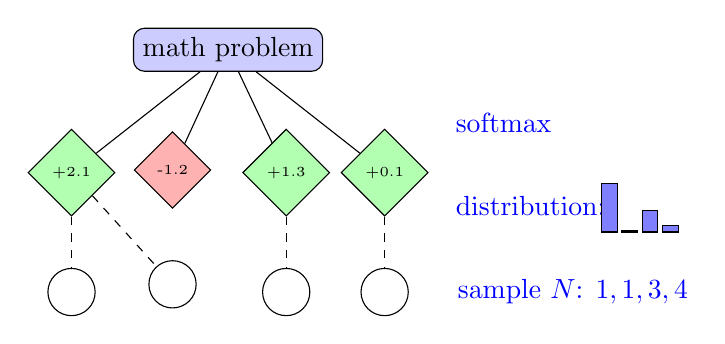
\begin{tikzpicture}
    % Define styles
    \tikzstyle{problem} = [rectangle, draw=black, fill=blue!20, rounded corners, minimum width=2cm, minimum height=0.5cm]
    \tikzstyle{node} = [circle, draw=black, minimum size=8mm, inner sep=0mm]
    \tikzstyle{selected} = [diamond, draw=black, fill=green!30, minimum size=6mm]
    \tikzstyle{unselected} = [diamond, draw=black, fill=red!30, minimum size=6mm]
    \tikzstyle{final} = [circle, draw=black, minimum size=6mm]
    \tikzstyle{bar} = [rectangle, draw=black, fill=blue!50]
    
    % Nodes
    \node[problem] (root) {math problem};
    
    \node[selected] (n1) [below left=1.0cm and 0.5cm of root] {\tiny +2.1};
    \node[unselected] (n2) [below left=1.0cm and -0.75cm of root] {\tiny -1.2};
    \node[selected] (n3) [below right=1.0cm and -0.75cm of root] {\tiny +1.3};
    \node[selected] (n4) [below right=1.0cm and 0.5cm of root] {\tiny +0.1};
    
    \node[final] (f1) [below=0.65cm of n1] {};
    \node[final] (f2) [below=0.65cm of n2] {};
    \node[final] (f3) [below=0.65cm of n3] {};
    \node[final] (f4) [below=0.65cm of n4] {};
    
    % Edges
    \draw (root) -- (n1);
    \draw (root) -- (n2);
    \draw (root) -- (n3);
    \draw (root) -- (n4);
    
    \draw[dashed] (n1) -- (f1);
    \draw[dashed] (n1) -- (f2);
    \draw[dashed] (n3) -- (f3);
    \draw[dashed] (n4) -- (f4);
    
    % Annotations
    \node[above right=0.1cm and 0.5cm of n4] {\textcolor{blue}{softmax}};
    \node[right=0.5cm of f4] {\textcolor{blue}{sample $N$: $1, 1, 3, 4$}};

    % Bars for softmax values
    \node[below right=-0.1cm and 0.5cm of n4] {\textcolor{blue}{distribution:}};
    \node[below right=0.35cm and 2.45cm of n4] (b1) {};
    \node[right=0.01cm of b1] (b2) {};
    \node[right=0.01cm of b2] (b3) {};
    \node[right=0.01cm of b3] (b4) {};
    
    \draw[bar] ($(b1) + (-0.1,0)$) rectangle ($(b1) + (0.1,+0.617)$);
    \draw[bar] ($(b2) + (-0.1,0)$) rectangle ($(b2) + (0.1,+0.023)$);
    \draw[bar] ($(b3) + (-0.1,0)$) rectangle ($(b3) + (0.1,+0.277)$);
    \draw[bar] ($(b4) + (-0.1,0)$) rectangle ($(b4) + (0.1,+0.083)$);
\end{tikzpicture}
        \caption{Particle filtering uses the rewards to produce a softmax distribution and does stochastic expansion of $N$ based sampling.}
        \label{fig:pf}
    \end{subfigure}
    \hfill
    \begin{subfigure}[t]{0.48\textwidth}
        % \centering
        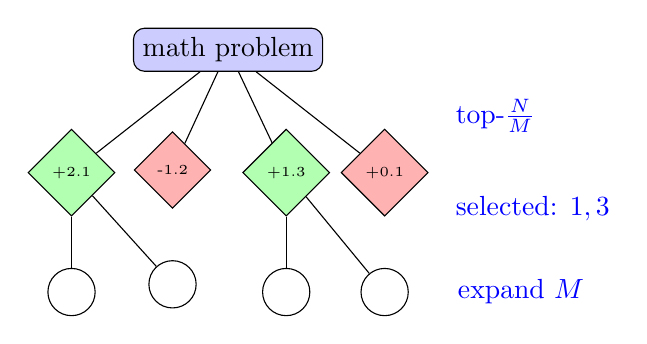
\begin{tikzpicture}
    % Define styles
    \tikzstyle{problem} = [rectangle, draw=black, fill=blue!20, rounded corners, minimum width=2cm, minimum height=0.5cm]
    \tikzstyle{node} = [circle, draw=black, minimum size=8mm, inner sep=0mm]
    \tikzstyle{selected} = [diamond, draw=black, fill=green!30, minimum size=6mm]
    \tikzstyle{unselected} = [diamond, draw=black, fill=red!30, minimum size=6mm]
    \tikzstyle{final} = [circle, draw=black, minimum size=6mm]
    
    % Nodes
    \node[problem] (root) {math problem};
    
    \node[selected] (n1) [below left=1cm and 0.5cm of root] {\tiny +2.1};
    \node[unselected] (n2) [below left=1cm and -0.75cm of root] {\tiny -1.2};
    \node[selected] (n3) [below right=1cm and -0.75cm of root] {\tiny +1.3};
    \node[unselected] (n4) [below right=1cm and 0.5cm of root] {\tiny +0.1};
    
    \node[final] (f1) [below=0.65cm of n1] {};
    \node[final] (f2) [below=0.65cm of n2] {};
    \node[final] (f3) [below=0.65cm of n3] {};
    \node[final] (f4) [below=0.65cm of n4] {};
    
    % Edges
    \draw (root) -- (n1);
    \draw (root) -- (n2);
    \draw (root) -- (n3);
    \draw (root) -- (n4);
    
    \draw (n1) -- (f1);
    \draw (n1) -- (f2);
    \draw (n3) -- (f3);
    \draw (n3) -- (f4);
    
    % Annotations
    \node[above right=0.1cm and 0.5cm of n4] {\textcolor{blue}{top-${N \over M}$}};
    \node[below right=-0.1cm and 0.5cm of n4] {\textcolor{blue}{selected: $1, 3$}};
    \node[right=0.5cm of f4] {\textcolor{blue}{expand $M$}};
\end{tikzpicture}
        \caption{Beam search treats the rewards as exact and performs deterministic expansion based on beam size $N$ and beam width $M$.}
        \label{fig:bs}
    \end{subfigure}
    \caption{A side-by-side comparison between particle filtering and its closet search-based counterpart, beam search.
    Compared with beam search in \figref{fig:bs} where the selection and expansion is deterministic (implicitly assumes the rewards are correct), particle filtering in \figref{fig:pf} trust the rewards with uncertainty and propagate the expansion via sampling.
    A more detailed, step-by-step version of particle filtering can be found in \figref{fig:pf-detailed} of \appref{app:alg}.}
    \label{fig:illustration}
    \vspace{-1.5em}
\end{figure}
% \begin{figure*}[t]
%     \centering
%     \includegraphics[width=\linewidth]{figures/image (8).png}
%     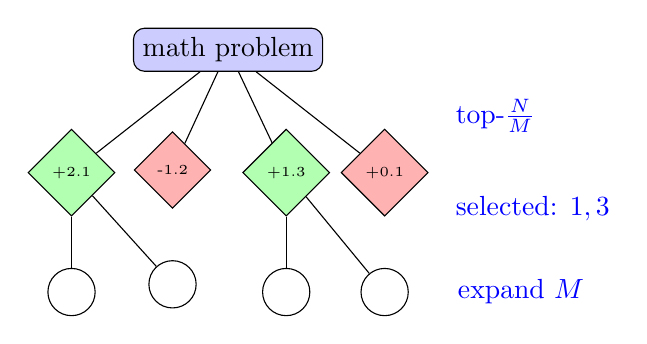
\begin{tikzpicture}
    % Define styles
    \tikzstyle{problem} = [rectangle, draw=black, fill=blue!20, rounded corners, minimum width=2cm, minimum height=0.5cm]
    \tikzstyle{node} = [circle, draw=black, minimum size=8mm, inner sep=0mm]
    \tikzstyle{selected} = [diamond, draw=black, fill=green!30, minimum size=6mm]
    \tikzstyle{unselected} = [diamond, draw=black, fill=red!30, minimum size=6mm]
    \tikzstyle{final} = [circle, draw=black, minimum size=6mm]
    
    % Nodes
    \node[problem] (root) {math problem};
    
    \node[selected] (n1) [below left=1cm and 0.5cm of root] {\tiny +2.1};
    \node[unselected] (n2) [below left=1cm and -0.75cm of root] {\tiny -1.2};
    \node[selected] (n3) [below right=1cm and -0.75cm of root] {\tiny +1.3};
    \node[unselected] (n4) [below right=1cm and 0.5cm of root] {\tiny +0.1};
    
    \node[final] (f1) [below=0.65cm of n1] {};
    \node[final] (f2) [below=0.65cm of n2] {};
    \node[final] (f3) [below=0.65cm of n3] {};
    \node[final] (f4) [below=0.65cm of n4] {};
    
    % Edges
    \draw (root) -- (n1);
    \draw (root) -- (n2);
    \draw (root) -- (n3);
    \draw (root) -- (n4);
    
    \draw (n1) -- (f1);
    \draw (n1) -- (f2);
    \draw (n3) -- (f3);
    \draw (n3) -- (f4);
    
    % Annotations
    \node[above right=0.1cm and 0.5cm of n4] {\textcolor{blue}{top-${N \over M}$}};
    \node[below right=-0.1cm and 0.5cm of n4] {\textcolor{blue}{selected: $1, 3$}};
    \node[right=0.5cm of f4] {\textcolor{blue}{expand $M$}};
\end{tikzpicture}
%     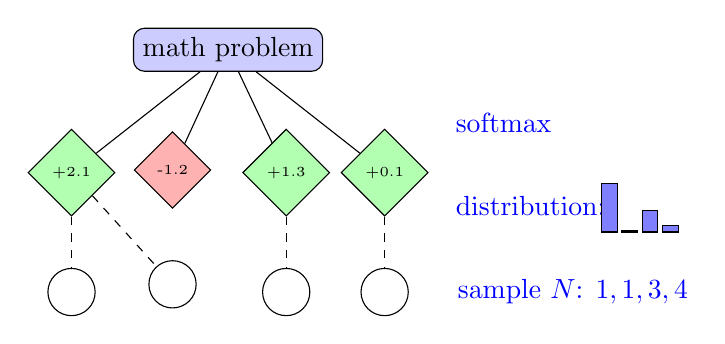
\begin{tikzpicture}
    % Define styles
    \tikzstyle{problem} = [rectangle, draw=black, fill=blue!20, rounded corners, minimum width=2cm, minimum height=0.5cm]
    \tikzstyle{node} = [circle, draw=black, minimum size=8mm, inner sep=0mm]
    \tikzstyle{selected} = [diamond, draw=black, fill=green!30, minimum size=6mm]
    \tikzstyle{unselected} = [diamond, draw=black, fill=red!30, minimum size=6mm]
    \tikzstyle{final} = [circle, draw=black, minimum size=6mm]
    \tikzstyle{bar} = [rectangle, draw=black, fill=blue!50]
    
    % Nodes
    \node[problem] (root) {math problem};
    
    \node[selected] (n1) [below left=1.0cm and 0.5cm of root] {\tiny +2.1};
    \node[unselected] (n2) [below left=1.0cm and -0.75cm of root] {\tiny -1.2};
    \node[selected] (n3) [below right=1.0cm and -0.75cm of root] {\tiny +1.3};
    \node[selected] (n4) [below right=1.0cm and 0.5cm of root] {\tiny +0.1};
    
    \node[final] (f1) [below=0.65cm of n1] {};
    \node[final] (f2) [below=0.65cm of n2] {};
    \node[final] (f3) [below=0.65cm of n3] {};
    \node[final] (f4) [below=0.65cm of n4] {};
    
    % Edges
    \draw (root) -- (n1);
    \draw (root) -- (n2);
    \draw (root) -- (n3);
    \draw (root) -- (n4);
    
    \draw[dashed] (n1) -- (f1);
    \draw[dashed] (n1) -- (f2);
    \draw[dashed] (n3) -- (f3);
    \draw[dashed] (n4) -- (f4);
    
    % Annotations
    \node[above right=0.1cm and 0.5cm of n4] {\textcolor{blue}{softmax}};
    \node[right=0.5cm of f4] {\textcolor{blue}{sample $N$: $1, 1, 3, 4$}};

    % Bars for softmax values
    \node[below right=-0.1cm and 0.5cm of n4] {\textcolor{blue}{distribution:}};
    \node[below right=0.35cm and 2.45cm of n4] (b1) {};
    \node[right=0.01cm of b1] (b2) {};
    \node[right=0.01cm of b2] (b3) {};
    \node[right=0.01cm of b3] (b4) {};
    
    \draw[bar] ($(b1) + (-0.1,0)$) rectangle ($(b1) + (0.1,+0.617)$);
    \draw[bar] ($(b2) + (-0.1,0)$) rectangle ($(b2) + (0.1,+0.023)$);
    \draw[bar] ($(b3) + (-0.1,0)$) rectangle ($(b3) + (0.1,+0.277)$);
    \draw[bar] ($(b4) + (-0.1,0)$) rectangle ($(b4) + (0.1,+0.083)$);
\end{tikzpicture}
%     \caption{Particle Filtering for Inference Scaling. We initialize $x$ particles with the "first step" of an answer to a question. At every step, each particle $p_i$ is given a score $s_i^t$ by the PRM, which is then used as a weight $w_i^t$ to determine how likely that particle is to be resampled (evolved via a solid line) at the next step. A particle is deemed "active" (green, in this diagram) until it generates an <EOS> token, after which it is still able to be resampled (evolved via a dashed line) but is not evolved further. This process continues until all particles have completed their answers and become inactive (filled yellow). \todokai{make new plot}}
%     \label{fig:illustration}
% \end{figure*}
\setlength{\textfloatsep}{4pt}
\begin{algorithm}[t]
\caption{Particle Filtering for Inference-Time Scaling}\label{alg:pf}
\begin{algorithmic}
\State \textbf{Input}: the number of particles $N$, a reward model $\hat{r}$, a LLM $p_M$ and the prompt $c$
\State Initialize $N$ particles $\{x_1^{(i)} \sim p_M(\cdot \mid c)\}_{i=1}^N$
\State $t \gets 1$
\While{not all particles stop} 
    \State Update rewards $\mathbf{w} = [\hat{r}(x_{1:t}^{(1)}), \dots, \hat{r}(x_{1:t}^{(N)})]$
    \State Compute softmax distribution $\theta = \mathrm{softmax}(\mathbf{w})$
    \State Sample indices $\{j_t^{(i)}\}_{i=1}^N  \sim \mathbb{P}_t(j=i) = \theta_i$
    \State Update the set of particles as $\{x_{1:t}^{(j_t^{(i)})}\}_{i=1}^N$
    \State Transition $\{x_{t+1}^{(i)} \sim p_M(\cdot \mid c, x_{1:t}^{(i)})\}_{i=1}^N$
    \State $t \gets t + 1$
\EndWhile
\State \textbf{Return}: the set of particles in the end
\end{algorithmic}
\end{algorithm}
\setlength{\textfloatsep}{20pt}

% Our method introduces a dynamic framework in which multiple hypotheses, each represented as a particle, are explored simultaneously across iterative steps, as illustrated in \figref{fig:illustration}.
% \begin{figure*}[t]
%     \centering
%     \includegraphics[width=\linewidth]{figures/image (8).png}
%     \caption{Particle Filtering for Inference Scaling. We initialize $x$ particles with the "first step" of an answer to a question. At every step, each particle $p_i$ is given a score $s_i^t$ by the PRM, which is then used as a weight $w_i^t$ to determine how likely that particle is to be resampled (evolved via a solid line) at the next step. A particle is deemed "active" (green, in this diagram) until it generates an <EOS> token, after which it is still able to be resampled (evolved via a dashed line) but is not evolved further. This process continues until all particles have completed their answers and become inactive (filled yellow).}
%     \label{fig:illustration}
% \end{figure*}
% The process operates as follows: 

% 1. We begins by initializing $n$ particles, each storing the first "step" of an answer, $h_i^0$. Here, $h_i^0$ represents the hypothesis of the $i$th particle at the step $t=0$. These steps are determined automatically through stop-token delimiters. 

% 2. At each step $t$ of the process, the PRM $R(h)$ evaluates the answers ("hypotheses") generated by the current set of particles, generating a set of scores. 
% $$s_i^t = R(h_i^t), \forall i \in {1, 2, ..., n}$$
% The PRM scores are transformed into a probability distribution over particles by applying a softmax function to the PRM scores, effectively assigning a weight $w_i^t$ to each particle that reflects its relative promise according to the reward model. 
% $$w_i^t = \frac{exp(s_i^t)}{\sum_{j=1}^{n} exp(s_j^t}\forall i \in {1, 2, ..., n}$$
% Notably, these weights do not blindly guide the selection of high-reward particles at every stage of our search - they also retain a degree of stochasticity that \textit{encourages exploration} of underexplored regions of the sample space - explorations that lead to the discovery of higher value answers later on. 

% 3. Once the particle weights have been computed, our framework resamples the aprticle set for the next step. THe resampling procedure is informed by the computed weights, where higher weighted particles are mroe likely to propagate their hypotheses into subsequent steps, but lower weighted particles retain a nonzero probability of being selected. 
% $$h_i^{t+1} \sim \text{Propagate}((h_i^t, w_i^t)_{i=1}^n)$$
% This mechanism, inspired by particle filtering techniques in Bayesian inference, ensures that the search process maintains a balance between exploiting promising hypotheses and exploring less-certain regions that may yield novel solutions. 

% 4. After resampling, each particle is unrolled by using the model $M$ to generate the next segment of its corresponding answer, effectively extending the hypotheses represented in the particle set. 
% $$h_i^{t+1} = \text{Sample Next Step}(M(h_i^t))$$
% This iterative process—evaluation, weighting, resampling, and unrolling—continues until all particles have generated complete answers, at which point the process terminates.

% By maintaining a diverse population of particles and dynamically adjusting their weights at each step, our method allows a level of flexibility that is absent in traditional strategies, such as greedy search or beam search. In general, the ability to guide exploration using PRM-based scores allows the framework to harness the strengths of reward models without being limited by their flaws. 

% Importantly, this approach ensures that inference scaling remains fruitful within smaller compute budgets, as the resampling and unrolling operations are computationally efficient and can be parallelized across particles. 

% - explain method: diagram of particle filtering approach 

\subsubsection{Multiple iterations and parallel chains}\label{sec:method-pg-pt}

The PF approach to inference-time scaling can be used to define a MCMC kernel that enables two new types of scaling: multiple iterations of complete answers inspired by PG and parallel simulations inspired by parallel tempering.

\textbf{Particle Gibbs} is a type of MCMC algorithm that uses PF as a transition kernel \citep{andrieu2010particlemarkov}. 
Specifically, at each iteration, PG samples a new set of particles  using PF with a reference particle from the previous iteration. 
This integration combines the efficiency of PF with the theoretical guarantees of MCMC, making PG suitable for high-dimensional or challenging posterior distributions.
The adaption of PG to inference-time scaling is essentially a multi-iteration extension of the PF algorithm presented, which works as follows:
For each iteration, we run a modified PF step with an additional sampling step to sample 1 reference particle according to \eqref{eq:resampling-dist}.
For any PF step that is not the initial step, the PF is executed with a reference particle: This reference particle is never replaced during the resampling step, but its partial trajectory can still be forked during resampling.
We detail the PG version of inference-time scaling in \algref{alg:pg} of \appref{app:alg}.
Note that typically, a reasonably large number of particles is needed to show the benefits of multiple iterations, which we also confirm in our results in \secref{sec:res-ablation}.

\paragraph{Parallel tempering}
In parallel tempering (aka replica exchange MCMC sampling), multiple MCMC chains run in parallel at different temperatures and swap the states to allow better exploration.
The key idea is that the chain running in high temperature can explore better, e.g.~traversing between different modes of the target, and the swap makes it possible to let the low temperature chain exploit the new region found by the other chain.
We detail the complete parallel tempering version of inference-time scaling in \algref{alg:pt} of \appref{app:alg} while we only explore a special case of it (multiple chains with single iteration) in our experiments.

\section{Evaluation}

We thoroughly evaluate our proposed methods in this section. 
We detail our experimental setup in \secref{sec:res-setup} and start with highlighted results on comparison with other closed-source models and competitive inference-time scaling methods with open-source models (\secref{sec:res-main}).
We then study how the main algorithm, particle filtering, scales with more computation and compare it with its competitors (\secref{sec:res-scaling}).
We further perform an extensive ablation study on key algorithmic choices like reward models, reward aggregation and LLM temperatures (\secref{sec:res-ablation}).
We finally study different possible allocations of the computation budget through iterative and parallel extensions (\secref{sec:res-alloc}).

\subsection{Setup}\label{sec:res-setup}

\paragraph{Models}
We consider two types of open-source small language models (SLMs) as our policy models for generating solutions.
The first is general-purpose models, of which we used Llama-3.2-1B-Instruct and Llama-3.1-8B-Instruct \citep{llama3}.
The second is math-specialized models, where we used Qwen2.5-Math-1.5B-Instruct and Qwen2.5-Math-7B-Instruct \citep{qwen_2_5}.
These small models are well-suited for inference-time scaling, enabling efficient exploration of multiple trajectories.

\paragraph{Process Reward Models}
To guide our policy models, we utilized Qwen2.5-Math-PRM-7B \citep{prmlessons}, a 7B process reward model. 
We selected this model because it demonstrated superior performance compared to other PRMs we tested, including Math-Shepherd-mistral-7b-prm \citep{wang2024mathshepherdverifyreinforcellms}, Llama3.1-8B-PRM-Deepseek-Data \citep{xiong2024rlhflowmath}, and EurusPRM-Stage2 \citep{primerm}. 
This result as an ablation study is provided in \secref{sec:res-ablation}, where we also study the different ways to aggregate step-level rewards from PRMs discussed in \secref{sec:method-pf}.

% Interestingly, we tested the Qwen PRM both for its original purpose as a true Process Reward Model and repurposed as an Outcome Reward Model. When used as a true Process Reward Model, the PRM is given the question and a list of steps that the policy model has generated so far. It calculates scores for each step of the process, of which we select the last score (a practice that was introduced and evaluated in \citet{beeching2024scalingtesttimecompute}). When used as an ORM, the Process Reward Model is given a question and a string that contains the concatenated steps that the policy model has generated thus far. It generates a score, which we then convert into a weight to use during the resampling process. We compare various reward models as well as the two configurations of the PRM in the ablation study shown in Figure \ref{fig:rm_comparison} below. 

\paragraph{Baselines}
\begin{tightlist}
    \item Pass@1: single greedy generation from the model, serving as the ``bottom-line'' performance.
    % \item Pass@64: results of any of the 64 generations is correct, serving as an approximate ``upper bound'' performance.
    \item BoN/WBoN \citep{brown2024largelanguage}: (weighted) best-of-N is the most straightforward inference-time scaling method using reward models.
    \item DVTS \citep{beeching2024scalingtesttimecompute}: a parallel extension of beam search that improves the exploration hence overall scaling performance.\footnote{We only consider DVTS but not beam search itself for two reasons. First, it has been reported by \citet{beeching2024scalingtesttimecompute} to have a better performance than beam search when the budget is more than 16. Second, the implementation of beam search from the official release by \citet{beeching2024scalingtesttimecompute} is slower than DVTS on the same budget.}
\end{tightlist}

\paragraph{Datasets}
To evaluate our methods and baselines, we consider 
% diverse mathematical benchmarks spanning multiple domains and difficulty levels. Our evaluation datasets include 
widely-used datasets spanning multiple domains and difficulty levels and challenging benchmarks, ensuring a robust assessment of the methods' performance across basic and advanced problem-solving and reasoning tasks.
\begin{tightlist}
    \item \textbf{MATH500} \citep{math500}: A dataset containing 500 high-difficulty competition-level problems from various mathematical domains.
    \item \textbf{AIME 2024} \citep{ai_mo_validation_aime}: A collection of 30 problems from the American Invitational Mathematics Examination (AIME I and II) 2024.
    % \item \textbf{GSM8K} \citep{cobbe2021trainingverifierssolvemath_gsm8k}: A benchmark of 8,000 grade-school-level math problems designed to test foundational reasoning abilities.
\end{tightlist}

\paragraph{Parsing and scoring}
To evaluate model-generated responses, we enforce a structured answer format using a system prompt (see \appref{app:example}). This prompt ensures that the final answer is enclosed within a \texttt{\textbackslash boxed\{\}} expression, facilitating automated extraction.
We provide a detailed version of our scoring process in \appref{app:eval}.


\subsection{Main results}\label{sec:res-main}
% We first show our main results on comparing our approach to a set of competitive baselines in \tabref{tab:maintable-performance}, where the results for all SLMs are based on a budget of 64 following \citet{} and Qwen2.5-Math-PRM-7B was used as the Reward Model.  
% Specifically, it was employed as an Outcome Reward Model (ORM) in the Weighted Best of N (WBoN) method and as a Process Reward Model (PRM) in other scaling methods.
% First, among all inference-time scaling methods, PF consistently performs the best with a noticeable margin.
% Second, for the Llama family, PF with Llama-3.1-8B-Instruct beats its larger version LLama-3.1-70B-Instruct on MATH500 and matches that on AIME 2024.
% Third, the best PF results with Qwen2.5-Math-1.5B-Instruct beats GPT-4o on both datasets.

We first present our main results, comparing our approach against a set of strong baselines in \tabref{tab:maintable-performance}. Inference-time scaling results are based on a budget of 64 samples, with Qwen2.5-Math-PRM-7B serving as the reward model. Specifically, it is used as an ORM in WBoN and as a PRM otherwise.
\begin{tightlist}
    \item Among all inference-time scaling methods, \textbf{PF consistently achieves the best performance}, outperforming other scaling methods by a significant margin.  
    \item \textbf{PF with Llama-3.1-8B-Instruct} outperforms its much larger counterpart, \textbf{Llama-3.1-70B-Instruct}, on \textbf{MATH500} and achieves parity on \textbf{AIME 2024}, demonstrating the efficiency of our approach.  
    \item The \textbf{best PF results with Qwen2.5-Math-1.5B-Instruct} surpass \textbf{GPT-4o} on both datasets, while coming very close to the \textbf{o1-preview} model on the MATH500 benchmark while the Qwen2.5-Math-7B-Instruct is able to match the performance of \textbf{o1-preview} on MATH500, further underscoring the effectiveness of our method.  
\end{tightlist}

% \begin{table}[ht]
% \centering
% \resizebox{\columnwidth}{!}{%
% \begin{tabular}{lccc}
% \toprule
% \textbf{Model}                                   & \textbf{MATH500} & \textbf{AIME 2024} & \textbf{GSM8K} \\
% \midrule
% \textbf{Frontier LLMs} \\
% GPT-4o                                          & 76.2       & -         & -       \\
% GPT-o1                                          & 87.0       & -         & -       \\
% \midrule
% \textbf{Open-Source LLMs} \\
% meta-llama/Llama-3.1-70B-Instruct               & 65.71   & -         & -       \\
% Qwen/Qwen2.5-Math-72B-Instruct                  & 79.6       & -         & -       \\
% % \midrule
% % \textbf{Open-Source SLMs}  (Qwen system prompt)\\
% % meta-llama/Llama-3.2-1B-Instruct               & 28.2   & 3.3       &  47.9     \\
% % meta-llama/Llama-3.1-8B-Instruct               & 50.4      & 6.7         &  84.5       \\
% % Qwen/Qwen2.5-7B-Instruct                       & 75.8     & 13.3         &  92.3    \\
% \midrule
% \textbf{Open-Source General SLMs}  \\
% meta-llama/Llama-3.2-1B-Instruct (Pass@1)               & 22.4(26.6)    &  0.0         &  43.5      \\
% meta-llama/Llama-3.2-1B-Instruct (WBoN)         & 46.6       & -         & -       \\
% meta-llama/Llama-3.2-1B-Instruct (DVTS)         & -       & -         & -       \\
% \rowcolor[HTML]{D9EAD3} % Light green
% meta-llama/Llama-3.2-1B-Instruct (Ours - PF)    & 57.2       & -         & -       \\
% meta-llama/Llama-3.1-8B-Instruct (Pass@1)              & 42 ( 50.0)     &  6.7      &   85.7      \\
% meta-llama/Llama-3.1-8B-Instruct (WBoN)         & 57.8       & -         & -       \\
% meta-llama/Llama-3.1-8B-Instruct (DVTS)         & -       & -         & -       \\
% \rowcolor[HTML]{D9EAD3} % Light green
% meta-llama/Llama-3.1-8B-Instruct (Ours - PF)    & -       & -         & -       \\
% % Qwen/Qwen2.5-7B-Instruct                       & 55(67.8)      &  6.7       &  86.6     \\
% \midrule
% \textbf{Open-Source Specialized SLMs} \\
% Qwen/Qwen2.5-Math-1.5B-Instruct (Pass@1)               &        & -         & -       \\
% Qwen/Qwen2.5-Math-1.5B-Instruct (WBoN)               & 66       & -         & -       \\
% Qwen/Qwen2.5-Math-1.5B-Instruct (DVTS)               & -       & -         & -       \\
% \rowcolor[HTML]{D9EAD3} % Light green
% Qwen/Qwen2.5-Math-1.5B-Instruct (Ours - PF)          & -       & -         & -       \\
% Qwen/Qwen2.5-Math-7B-Instruct (Pass@1)               &        & -         & -       \\
% Qwen/Qwen2.5-Math-7B-Instruct (WBoN)               &        & -         & -       \\
% Qwen/Qwen2.5-Math-7B-Instruct (DVTS)               & -       & -         & -       \\
% \rowcolor[HTML]{D9EAD3} % Light green
% Qwen/Qwen2.5-Math-7B-Instruct (Ours - PF)          & -       & -         & -       \\
% \bottomrule
% \end{tabular}%
% }
% \caption{Results of various LLMs on challenging math benchmarks, including MATH500, AIME 2024, and GSM8K. All inference scaling experiments were run with a budget of 16 generations per problem. The table highlights the performance of Inference Scaling methods, where Qwen/Qwen2.5-Math-PRM-7B was used as the Reward Model. Specifically, it was employed as an Outcome Reward Model (ORM) in the Weighted Best of N (WBoN) method and as a Process Reward Model (PRM) in other scaling methods. The models `Ours - PF` represent our Particle-Based Monte Carlo approach to inference-time scaling.}
% \label{tab:maintable-performance}
% \end{table}

% \begin{table}[ht]
% \centering
% \resizebox{\columnwidth}{!}{%
% \begin{tabular}{ll|ccc}
% \toprule
% \textbf{Model}                                   & \textbf{Method} & \textbf{MATH500} & \textbf{AIME 2024} & \textbf{GSM8K} \\
% \midrule
% \textbf{Closed-Source LLMs} \\
% GPT-4o                                          & -          & 76.2       & -         & -       \\
% GPT-o1                                          & -          & 87.0       & -         & -       \\
% \midrule
% \textbf{Open-Source LLMs} \\
% Llama-3.1-70B-Instruct               & -          & 62        & 16.7        &  70.3 \footnote{By using the Qwen-math system prompt, GSM8K accuracy improves to 94.8. The model's performance on the GSM8K task shows high sensitivity to system prompt selection.}      \\
% Qwen2.5-Math-72B-Instruct                  & -          & 84.0       & 26.7         & 95.7      \\
% \midrule
% \textbf{Open-Source SLMs} \\
% Llama-3.2-1B-Instruct               & Pass@1     & 25.2        & 0.0       & 44.5    \\
%                                                & WBoN       & 46.6       & -         & -       \\
%                                                & DVTS       & -          & -         & -       \\
%                                                & \rowcolor[HTML]{D9EAD3} Ours - PF  & 60.0       & -         & -       \\
% Llama-3.1-8B-Instruct               & Pass@1     & 48.2        & 6.7       & 84.5    \\
%                                                & WBoN       & 57.8       & -         & -       \\
%                                                & DVTS       & -          & -         & -       \\
%                                                & \rowcolor[HTML]{D9EAD3} Ours - PF  & 4morehours          & -         & -       \\
% \midrule
% \textbf{Open-Source Math SLMs} \\
% Qwen2.5-Math-1.5B-Instruct                & Pass@1     & 72.6         & 10.0        & 80.4      \\
%                                                & WBoN       & 66.0 (??)       & -         & -       \\
%                                                & DVTS       & -          & -         & -       \\
%                                                & \rowcolor[HTML]{D9EAD3} Ours - PF  & 85.0          & -         & -       \\
% Qwen2.5-Math-7B-Instruct                  & Pass@1     &  83.2       & 13.3        & 95.6       \\
%                                                & WBoN       & -          & -         & -       \\
%                                                & DVTS       & -          & -         & -       \\
%                                                & \rowcolor[HTML]{D9EAD3} Ours - PF  & 87.0          & -         & -       \\
% \bottomrule
% \end{tabular}
% }

% \begin{table}[ht]
% \centering
% \resizebox{\columnwidth}{!}{%
% \begin{tabular}{ll|cc}
% \toprule
% \textbf{Model}                                   & \textbf{Method} & \textbf{MATH500} & \textbf{AIME 2024} \\
% \midrule
% \textbf{Closed-Source LLMs} \\
% GPT-4o                                          & -          & 76.2       & -       \\
% GPT-o1                                          & -          & \textbf{87.0}       & -       \\
% \midrule
% \textbf{Open-Source LLMs} \\
% Llama-3.1-70B-Instruct               & -          & 62        & 16.7       \\
% Qwen2.5-Math-72B-Instruct                  & -          & 84.0       & 26.7       \\
% \midrule
% \textbf{Open-Source SLMs} \\
% Llama-3.2-1B-Instruct               & Pass@1     & 25.2        & 0.0       \\
%                                                & WBoN       & 46.6       & -       \\
%                                                & DVTS       & -          & -       \\
%                                                \rowcolor[HTML]{D9EAD3}&  Ours - PF  & 60.0       & -       \\
% Llama-3.1-8B-Instruct               & Pass@1     & 48.2        & 6.7       \\
%                                                & WBoN       & 57.8       & -       \\
%                                                & DVTS       & -          & -       \\
%                                                \rowcolor[HTML]{D9EAD3}&  Ours - PF  & 4morehours  & -       \\
% \midrule
% \textbf{Open-Source Math SLMs} \\
% Qwen2.5-Math-1.5B-Instruct                & Pass@1     & 72.6         & 10.0       \\
%                                                & WBoN       &    & -       \\
%                                                & DVTS       & -          & -       \\
%                                                \rowcolor[HTML]{D9EAD3}&  Ours - PF  & 85.0        & -       \\
% Qwen2.5-Math-7B-Instruct                  & Pass@1     & 79.6         & 13.3       \\
%                                                & WBoN       & -          & -       \\
%                                                & DVTS       & -          & -       \\
%                                                \rowcolor[HTML]{D9EAD3} & Ours - PF  & \textbf{87.0}        & -       \\
% \bottomrule
% \end{tabular}
\begin{table}[t]
\centering
\resizebox{\columnwidth}{!}{%
\begin{tabular}{ll|cc}
\toprule
\textbf{Model}                                   & \textbf{Method} & \textbf{MATH500} & \textbf{AIME 2024} \\
\midrule
\textbf{Closed-Source LLMs} \\
GPT-4o                                          & -          & 76.2       & 13.3         \\
o1-preview                                          & -          & \textit{\textbf{87.0}}       & \textit{\textbf{40.0}}         \\
Claude3.5-Sonnet                          & - & 78.3 & 16.0  \\  
\midrule
\textbf{Open-Source LLMs} \\
Llama-3.1-70B-Instruct               & -          & 65.7        & 16.6       \\
Qwen2.5-Math-72B-Instruct                  & -          & 82.0       & 30.0       \\                   
\midrule
\textbf{Open-Source SLMs} \\
Llama-3.2-1B-Instruct               & Pass@1     & 26.8        & 0.0       \\
                                               % & Pass@64       & -       & 30.6         \\
                                               & BoN         & 46.6          & 3.3           \\
                                               & WBoN       & 47.8       & 3.3         \\
                                               & DVTS       & 52.8          & 6.6         \\
                                               \rowcolor[HTML]{D9EAD3} & Ours - PF  & \textbf{59.6}       & \textbf{10.0}         \\\hline
Llama-3.1-8B-Instruct               & Pass@1     & 49.9        & 6.6       \\
                                               % & Pass@64       & -       & 40.0         \\
                                               & BoN         & 58.6          & 10.0           \\
                                               & WBoN       & 59.0       & 10.0         \\
                                               & DVTS       & 65.7          & 13.3         \\
                                               \rowcolor[HTML]{D9EAD3} & Ours - PF  & \textbf{74.4}  & \textbf{16.6}         \\
\midrule
\textbf{Open-Source Math SLMs} \\
Qwen2.5-Math-1.5B-Instruct                & Pass@1     & 70.0         & 10.0       \\
                                               % & Pass@64       & 95.2       & 40.0         \\
                                               & BoN         & 82.6           & 13.3           \\
                                               & WBoN       & 82.8           & 13.3         \\
                                               & DVTS       & 83.4           & 16.6         \\
                                               \rowcolor[HTML]{D9EAD3} & Ours - PF  & \textbf{85.4}        & \textbf{23.3}         \\\hline
Qwen2.5-Math-7B-Instruct                  & Pass@1     & 79.6         & 16.6       \\
                                               % & Pass@64       & 96.0       & 53.3         \\
                                            & BoN         & 83.0           & 20.0           \\
                                               & WBoN       & 84.6           & 20.0         \\
                                               & DVTS       & 85.4           & 20.0         \\
                                               \rowcolor[HTML]{D9EAD3} & Ours - PF  & \textit{\textbf{87.0}}        & \textbf{23.3}         \\
\bottomrule
\end{tabular}
} 
\caption{Results of various LLMs on MATH500 and AIME 2024 where \textbf{bold} indicates the best in each category and \textit{italic} indicates the overall best. The table highlights the performance of Inference Scaling methods, where Qwen2.5-Math-PRM-7B was used as the Reward Model.  
Each inference scaling methods were run with a computational budget of 64 model generations. Notably, the Qwen2.5-Math-7B model, when scaled with inference-time compute, achieves performance on par with o1-preview in MATH500, further showcasing the power of inference-time scaling for competitive performance with smaller models.}
\label{tab:maintable-performance}
\vspace{-1.5em}
\end{table}

\subsection{Scaling with inference-time compute}\label{sec:res-scaling}
We now zoom in on how PF scales with inference-time compute.
\Figref{fig:llama_qwen_comparison} shows the change of performance (in terms of accuracy) with an increasing computation budget ($N=1, 2, 4, 8, 16, 32, 64, 128$) for all SLMs we consider.
As we can see, PF scales 4--16x faster than the next best competitor DVTS, % e.g.~PF requires a budget of only 8 generations to reach the performance that DVTS achieves at 32 generations,  requires a budget of 32 to reach  performance of PF with a budget of 8 with LLama-3.2-1B-Instruct and requires a budget of 128 to reach the performance of PF with a budget of 8 with LLama-3.1-8B-Instruct.
e.g.~DVTS requires a budget of 32 to reach the same performance of PF with a budget of 8 with LLama-3.2-1B-Instruct and requires a budget of 128 to reach the performance of PF with a budget of 8 with LLama-3.1-8B-Instruct.
% \looseness=-1

\subsection{Ablation study}\label{sec:res-ablation}

% In this section we perform ablation study on a few critical algorithm choices we make through the experiments.

\paragraph{Performance of different PRMs}
To investigate the impact of the choice of PRM on our method, in Figure \ref{fig:rm_comparison} we present the results of an ablation study on a subset of 100 questions from the MATH500 dataset, where we compare the accuracy of our method across various reward functions as the number of particles increases.
\begin{figure}[t]
    \centering
    \includegraphics[width=0.77\columnwidth]{figures/rm_comparison.pdf}
    \caption{Results of ablation on 100 question subset comparing the performance of PF across various PRMs. We find that the Qwen PRM scales the most effectively across generations.}
    \label{fig:rm_comparison}
    \vspace{-1em}
\end{figure}
% prev caption - Effect of PRMs on our method evaluated on a 100-question subset of the MATH500 dataset. The figure shows that our method scales effectively across different PRMs, including Qwen2.5-Math-PRM-7B, Llama3.1-8B-PRM-Deepseek-Data, and EurusPRM-Stage2.
Qwen2.5-Math-PRM-7B consistently outperforms other models, making it the natural choice for our main results. Interestingly, while EurusPRM-Stage2 performs relatively poorly with smaller budgets, it gradually improves and eventually matches Qwen2.5-Math-PRM-7B at higher budgets.

\paragraph{Reward aggregation within PRMs}

As mentioned in \secref{sec:method-pf} and reported by many previous works \citep{zhang2025lessonsdeveloping}, there exist multiple ways to use PRMs to calculate reward scores which   can have large impact on final performance. 
\Figref{fig:aggregation_comparison} studies 3 existing ways to use a set of PRM scores---using the \textit{last} reward, the \textit{minimum} reward, and the \textit{product} of all the rewards. We also study ``Model Aggregation'', through which we use the PRM as an ORM with partial answers. 
\begin{figure}[t]
    \centering
    \includegraphics[width=0.77\linewidth]{figures/agg_comparison.pdf}
    \caption{
    Effect of different aggregation strategies for the process reward model Qwen2.5-Math-PRM-7B, evaluated on a 100-question subset of the MATH500 dataset. The plot compares the commonly used aggregation strategies—Min, Last, and Product—against our proposed Model Aggregation method. 
    }
    \label{fig:aggregation_comparison}
    \vspace{-1.5em}
\end{figure}
As we can see, using Model Aggregation---in essence, feeding into a PRM the entire partial answer alongside the question - scales the best with an increasing budget.\looseness=-1

\paragraph{Controlling the state transition---temperatures in LLM generation}

We investigate the effect of different LM sampling temperatures on the scaling of our method across different numbers of particles. The results of our ablation study on a 100 question subset of MATH questions are shown in Figure \ref{fig:model_temp_sweep_plot}.
\begin{figure}[t]
    \centering
    \includegraphics[width=0.77\linewidth]{figures/model_temp_comparison.pdf}
    \caption{Results of using Llama 3.2 1B as our policy model across temperatures (0.4, 0.6, 0.8, 1.0, 1.2,  and 1.4) and particle numbers (1, 2, 4, 8, 16, and 32).}
    \label{fig:model_temp_sweep_plot}
    \vspace{-1em}
\end{figure}
Our findings indicate that the commonly used range of llm temperature of 0.4--1.0 performs well, with minimal variations in accuracy across different budgets. Similar to \citet{beeching2024scalingtesttimecompute}, we set the temperature to 0.8 for all our experiments. 
% Our results show that our method is robust to model sampling temperatures as the scaling curves mostly overlap with each other.
% Our results show that different model sampling temperatures is optimal for each number of particles. Motivated by the discrepancies between various sampling temperatures, we tested a variant of our method that runs individual particles within a run at different temperatures in \secref{sec:res-alloc}.

\subsection{Budget allocation over iterations and parallelism}\label{sec:res-alloc}

The multi-iteration and parallel-chain extensions introduced in \secref{sec:method-pg-pt} provides two more axes to spend computation in addition to the number of particles.
We now explore how different ways to allocate budgets changes the performance.
Specifically, we study for a fixed budget $N \times T \times M$, how the combination of $N,T,M$ can yield the best performance, where $N$ is the number of particles, $T$ is the number of iterations, and $M$ is the number of parallelism.

\paragraph{Allocating budget between $N$ and $T$}

\begin{figure}
    \centering
    \includegraphics[width=0.77\linewidth]{figures/pg_analysis.pdf}
    \caption{Comparison of PF and Particle Gibbs with different numbers of iterations, evaluated on a 100-question subset of the MATH-500 dataset using Llama-3.2-1B-Instruct as the policy model.}
    \label{fig:pg_analysis}
    \vspace{-1.5em}
\end{figure}

Figure \ref{fig:pg_analysis} shows results of Llama-3.2 1B model when configured with various test-time compute budget allocations. Although the plot shows that various Particle Gibbs configurations do not have a marked benefit over an equivalently budgeted particle filtering run, a PG experiment with 16 particles and 4 iterations powered by a Qwen 2.5 7B Math Instruct policy model achieved a 87.2\% accuracy on MATH500, beating o1 performance. Configurations with larger $N$ values typically do better than equivalently budgeted runs with less particles.

\paragraph{Allocating budget between $N$ and $M$}

\Figref{fig:pt_comparison} shows PF and 3 PT configurations over a set of increasing numbers of budgets.
\begin{figure}[t]
    \centering
    \includegraphics[width=0.77\columnwidth]{figures/pt_comparison.pdf}
    \caption{
    Comparison of PF and PT with different particle group sizes, evaluated on a 100-question subset of the MATH500 dataset using Llama-3.2-1B-Instruct as the policy model.}
    \label{fig:pt_comparison}
    \vspace{-1.5em}
\end{figure}
First, as we can see, for any fixed $N$, increasing $M$ also improves the performance.
This may be helpful when combining batch generation with distributed computing.
Second, PT with $N=16$ has a better overall scaling than PF.
This indicates that there is some optimal budget allocation over parallel chains that can further improve the overall performance of our main results.

We leave the exploration over the optimal configuration of $N,T,M$ jointly as a future work.


% \todoshiv{add more info about this method}

% \paragraph{Effect of Particle Initialization - Softmax Temperature}
% \todokai{optional}
% \begin{figure}
%     \centering
%     \includegraphics[width=\linewidth]{softmaxtemp_sweep_math500_100sbset.png}
%     \caption{softmax temp sweep - needs to be replaced by PDF verison}
%     \label{fig:enter-label}
% \end{figure}

% \paragraph{Effect of Particle Initialization - Model Mixture}

% Current Plots: 


% - policy models: 
%     - llama 1b
%     - qwen 1.5b
%     - llama 8b
%     - llama 70b 
%     - qwen 72b

% - reward models:    
%     - deepseek
%     - mathshephard 
%     - prime e


% - other methods to compare against: 
%     - dvts
%     - 
%     - 

% - ablations in our own framework: 
%     - particle init
%     - temperature init
%     - PF vs slightly adjusted split apart PF stuff 


\section{Conclusion}
In this paper, we introduce a set of inference-time scaling algorithms with PRMs that leverage particle-based Monte Carlo methods. Our evaluation demonstrates that these algorithms consistently outperform search-based approaches by a significant margin.

However, inference-time scaling comes with computational challenges. Hosting and running a reward model often introduces high latency, making the process more resource-intensive. Additionally, for smaller models, extensive prompt engineering is often required to ensure outputs adhere to the desired format. Finally, hyperparameters such as temperature are problem-dependent and may require extensive tuning across different domains.

We hope that the formal connection of inference scaling to probabilistic modeling that we established in this work will lead to systematic solutions for the current limitations of these methods and pave the way for bringing advanced probabilistic inference algorithms into LLM inference-time scaling in future work.

\newpage 

% REMOVING FOR ARXIV
% \section*{Impact Statement}
% This paper presents work whose goal is to advance the field of Machine Learning. There are many potential societal consequences of our work, none which we feel must be specifically highlighted here.




% Acknowledgements should only appear in the accepted version.
% \section*{Acknowledgements}

\bibliography{main}
\bibliographystyle{icml2021}

%%%%%%%%%%%%%%%%%%%%%%%%%%%%%%%%%%%%%%%%%%%%%%%%%%%%%%%%%%%%%%%%%%%%%%%%%%%%%%%
%%%%%%%%%%%%%%%%%%%%%%%%%%%%%%%%%%%%%%%%%%%%%%%%%%%%%%%%%%%%%%%%%%%%%%%%%%%%%%%
% APPENDIX
%%%%%%%%%%%%%%%%%%%%%%%%%%%%%%%%%%%%%%%%%%%%%%%%%%%%%%%%%%%%%%%%%%%%%%%%%%%%%%%
%%%%%%%%%%%%%%%%%%%%%%%%%%%%%%%%%%%%%%%%%%%%%%%%%%%%%%%%%%%%%%%%%%%%%%%%%%%%%%%
\newpage
\appendix
\onecolumn
\section{Appendix}

\subsection{Algorithm details}\label{app:alg}

\begin{figure}[t][h]
    \centering
    \includegraphics[width=\linewidth]{figures/particle_filtering_figures-cropped.pdf}
    \caption{Particle filtering for inference scaling in details. We initialize $x$ particles with the "first step" of an answer to a question. At every step, each particle $p_i$ is given a score $s_i^t$ by the PRM, which is then used as a weight $w_i^t$ to determine how likely that particle is to be resampled (evolved via a solid line) at the next step. A particle is deemed "active" (green, in this diagram) until it generates an \texttt{\textlangle EOS\textrangle} token, after which it is still able to be resampled (evolved via a dashed line) but is not evolved further. This process continues until all particles have completed their answers and become inactive (filled yellow).}
    \label{fig:pf-detailed}
\end{figure}

\begin{algorithm}[t]
\caption{Particle Gibbs for Inference-Time Scaling}\label{alg:pg}
\begin{algorithmic}
\State \textbf{Input}: same as \algref{alg:pf} with the number of Gibbs iterations $T$
\State Run \algref{alg:pf} to get a set of particles $\{x_{1:t}^{(i)}\}_{i=1}^N$
\For{$j=1, \dots, T$}
    \State Compute rewards $\mathbf{w} = [\hat{r}(x_{1:t}^{(1)}), \dots, \hat{r}(x_{1:t}^{(N)})]$
    \State Compute softmax distribution $\theta = \mathrm{softmax}(\mathbf{w})$
    \State Sample reference particle $x_{1:t}^{\text{ref}} := x_{1:t}^{(j)}$ where $j \sim \mathbb{P}(j=i) = \theta_i$
    \State Initialize $N-1$ particles $\{x_1^{(i)} \sim p_M(\cdot \mid c)\}_{i=1}^{N-1}$
    \State $t \gets 1$
    \While{not all particles stop} 
        \State Update $\mathbf{w} = [\hat{r}(x_{1:t}^{(1)}), \dots, \hat{r}(x_{1:t}^{(N-1)}), \hat{r}(x_{1:t}^{\text{ref}})]$
        \State Compute softmax distribution $\theta = \mathrm{softmax}(\mathbf{w})$
        \State Sample indices $\{j_t^{(i)}\}_{i=1}^N  \sim \mathbb{P}_t(j=i) = \theta_i$
        \State Update the set of particles as $\{x_{1:t}^{(j_t^{(i)})}\}_{i=1}^N$
        \State Transition $\{x_{t+1}^{(i)} \sim p_M(\cdot \mid c, x_{t+1}^{(i)})\}_{i=1}^N$
        \State $t \gets t + 1$
    \EndWhile
\EndFor
\State \textbf{Return}: the set of particles in the end
\end{algorithmic}
\end{algorithm}

For a set of parallel chains with temperatures $T_1 > T_2 > \dots$, at each iteration, we swap the states of every pair of neighboring chains $k, k+1$ with the following probability
\begin{equation}\label{eq:pt-swap-prob}
A = \min\left(1, \frac{\pi_k(x^{(k+1)}) \pi_{k+1}(x^{(k)})}{\pi_k(x^{(k)}) \pi_{k+1}(x^{(k+1)})}\right),
\end{equation}
where $\pi_k, \pi_{k+1}$ are the two targets (with different temperatures) and $x_k, x_{k+1}$ are their states before swapping.
\begin{algorithm}[t]
\caption{Particle Gibbs with Parallel Tempering for Inference-Time Scaling}\label{alg:pt}
\begin{algorithmic}
\State \textbf{Input}: same as \algref{alg:pg} with the number of parallel chains $M$ and a list of temperature $T_1, \dots, T_M$
\For{$j=1, \dots, T$}
    \For{$k=1, \dots, M$}
        \If{$j = 1$}
            \State Run \algref{alg:pf} to get a set of particles $\{x_{1:t}^{(i)}\}_{i=1}^N$ for chain $k$
        \Else
            \State Initialize $N-1$ particles $\{x_1^{(i)} \sim p_M(\cdot \mid c)\}_{i=1}^{N-1}$
            \State $t \gets 1$
            \While{not all particles stop} 
                \State Update $\mathbf{w} = [\hat{r}(x_{1:t}^{(1)}), \dots, \hat{r}(x_{1:t}^{(N-1)}), \hat{r}(x_{1:t}^{\text{ref}})]$
                \State Compute softmax distribution $\theta = \mathrm{softmax}(\mathbf{w} / T_k)$
                \State Sample indices $\{j_t^{(i)}\}_{i=1}^N  \sim \mathbb{P}_t(j=i) = \theta_i$
                \State Update the set of particles as $\{x_{1:t}^{(j_t^{(i)})}\}_{i=1}^N$
                \State Transition $\{x_{t+1}^{(i)} \sim p_M(\cdot \mid c, x_{t+1}^{(i)})\}_{i=1}^N$
                \State $t \gets t + 1$
            \EndWhile
        \EndIf
        \State Compute rewards $\mathbf{w} = [\hat{r}(x_{1:t}^{(1)}), \dots, \hat{r}(x_{1:t}^{(N)})]$
        \State Compute softmax distribution $\theta = \mathrm{softmax}(\mathbf{w} / T_k)$
        \State Sample reference particle $x_{1:t}^{\text{ref}} := x_{1:t}^{(j)}$ where $j \sim \mathbb{P}(j=i) = \theta_i$
    \EndFor
    \For{$k=1, \dots, M-1$}
        \State Exchange the reference particle between chain $k$ and $k+1$ with probability according to \eqref{eq:pt-swap-prob}
    \EndFor
\EndFor
\State \textbf{Return}: $M$ set of particles in the end
\end{algorithmic}
\end{algorithm}

\subsection{Inference Prompt Template}\label{app:example}

\begin{tcolorbox}[colback=gray!10, colframe=gray!80, sharp corners, title=Evaluation System Prompt]\label{prompt_template}
\begin{verbatim}
Solve the following math problem efficiently and clearly:
    - For simple problems (2 steps or fewer):  
    Provide a concise solution with minimal explanation.

    - For complex problems (3 steps or more):
    Use this step-by-step format:
    
    ## Step 1: [Concise description]
    [Brief explanation and calculations]

    ## Step 2: [Concise description]
    [Brief explanation and calculations]

Regardless of the approach, always conclude with:

Therefore, the final answer is: $\boxed{answer}$. I hope it is correct.

Where [answer] is just the final number or expression that solves the problem.
\end{verbatim}
\end{tcolorbox}

\begin{tcolorbox}[colback=gray!10, colframe=gray!80, sharp corners, title=PRM Input Format]\label{code:prm}
\begin{verbatim}
## Step 1: [Concise description]
[Brief explanation and calculations]
<reward_token>
## Step 2: [Concise description]
[Brief explanation and calculations]
<reward_token>
## Step 3: [Concise description]
[Brief explanation and calculations]
<reward_token>
\end{verbatim}
\end{tcolorbox}

\begin{tcolorbox}[colback=gray!10, colframe=gray!80, sharp corners, title=ORM Input Format]\label{code:orm}
\begin{verbatim}
## Step 1: [Concise description]
[Brief explanation and calculations]
## Step 2: [Concise description]
[Brief explanation and calculations]
## Step 3: [Concise description]
[Brief explanation and calculations]
<reward_token>
\end{verbatim}
\end{tcolorbox}

\subsection{Evaluation details}\label{app:eval}

\paragraph{Parsing and scoring}
Following prior work on mathematical reasoning benchmarks \citep{qwen_2_5}, we apply their heuristic-based parsing and cleaning techniques to robustly extract the boxed expression. These heuristics account for variations in spacing, formatting inconsistencies, and other common artifacts observed in model outputs. For answer verification, we follow \citet{beeching2024scalingtesttimecompute} and convert responses to canonical form. Ground truth and generated answers are transformed from LaTeX into SymPy expressions, simplified for normalization, and converted back to LaTeX.
Exact match is determined using two criteria: numerical equality, where both expressions evaluate to the same floating-point value, and symbolic equality, where both are algebraically equivalent as SymPy expressions \citep{beeching2024scalingtesttimecompute}. Accuracy is then computed as the fraction of problems where the generated answer exactly matches the ground truth.

%%%%%%%%%%%%%%%%%%%%%%%%%%%%%%%%%%%%%%%%%%%%%%%%%%%%%%%%%%%%%%%%%%%%%%%%%%%%%%%
%%%%%%%%%%%%%%%%%%%%%%%%%%%%%%%%%%%%%%%%%%%%%%%%%%%%%%%%%%%%%%%%%%%%%%%%%%%%%%%


\end{document}

